\subsection{Electric Charges and Electric Fields} 

%\DTMnewdatestyle{dateupdated}{〈definition 〉

Answers to M\Alph{subsection} problems are on page \pageref{charges_prob_answers}.  \textbf{\textcolor{red}{Updated \DTMnow.}}

%--------------------------------------------------------------------------------------------------------------
\begin{Exercise}
Richard Feynman, a Nobel Prize-winning physicist, once noted that if two people stood an arm's length away from each other, and each person had just 1\% more electrons than protons, the force pushing them away from each other would be enough to lift the ``weight'' of the entire planet Earth.  
Do an order-of-magnitude calculation to determine whether this is true.  
(\textit{Hint: the fact that he won a Nobel Prize in physics should be your clue that it's probably true.}) 
\end{Exercise}

%--------------------------------------------------------------------------------------------------------------
\begin{Exercise}
Caitlin Clark and the Indiana Fever are playing two games against A'ja Wilson and the Las Vegas Aces.  
Suppose that there are two basketballs, one in Indianapolis and one in Las Vegas,  
and suppose that by some miracle, the basketball in Indianapolis suddenly loses all of its electrons, and the one in Las Vegas suddenly loses all of its protons.  
(We'll ignore for the moment that if this actually happened, each ball would instantly blow itself to smithereens.)  
Do an order-of-magnitude calculation to show that the attractive force between the two balls at this distance would be so great that all of the members of both teams working together wouldn't be strong enough to hold them apart.
\end{Exercise}
\begin{Answer}
My estimate for the force between the balls is $\sim 10^{11}$~N.  That's about 10 billion pounds of force!  
(How many pounds of force do you think you could apply to the ball if you were trying to hold it back?  
How would your answer change if your name was A'ja Wilson?) 
\end{Answer}

%--------------------------------------------------------------------------------------------------------------
\begin{Exercise}
The gravitational force between two objects of mass $m_1$ and $m_2$ is given by $\displaystyle F_G=\frac{Gm_1 m_2}{r^2}$, where the gravitational constant $G=6.67 \times 10^{-11}$~N$\cdot$m$^2$/kg$^2$.  In a hydrogen atom, the electron and the proton are separated by an average distance of one Bohr radius, or about $5 \times 10^{-11}$~m.  
Which force is stronger between the hydrogen's electron and the proton: the electrical force or the gravitational force?    
\end{Exercise}
\begin{Answer}
The electric force is about $2 \times 10^{39}$ times stronger than the gravitational force!
\end{Answer}

%--------------------------------------------------------------------------------------------------------------
\figuretoright{0.38}[scale=0.95]{M_problems/charges/charges_on_rod.pdf}{
\begin{Exercise}
Two small balls with positive charges $q_1=3q$ and $q_2=q$ are glued to the opposite ends of a horizontal insulating rod of length $d=1.50$~ m.  
The $q_1$ ball is at the origin.  
A third small ball, also charged, is free to slide back and forth on the rod.  

(a)~At what $x$ position is the third ball at equilibrium?
  
(b)~Can that equilibrium be a stable equilibrium? Explain.

\end{Exercise}
}\begin{Answer}
(a) 0.951 m (b) Hmmm... depends on the signs of the charges....
\end{Answer}

%--------------------------------------------------------------------------------------------------------------
\figuretoright{0.30}[scale=0.95]{M_problems/charges/triangle_charges.pdf}{
\begin{Exercise}
Three charged balls are on the corners of an equilateral triangle, as shown. 
What is the total electric force on the ball with the $7.00~\mu$C charge?
\end{Exercise}
\begin{Answer}
 0.872 N, 30$^\circ$ below the $x$ axis
\end{Answer}

%--------------------------------------------------------------------------------------------------------------
\begin{Exercise}
A regulation NHL hockey puck measures three inches across and one inch thick 
($R=3.81$~cm, $h=2.54$~cm).  Suppose that a particular puck carries a charge density $\rho$
that varies with the distance $r$ from the center of the puck\footnotemark ~according to
$$
\rho = (430~\text{nC/m}^2)\left(\frac{1}{r} \right) \sin \left( \pi \frac{r}{R} \right).
$$
What is the total charge $Q$ on the puck?

\end{Exercise}
}%END OF \figuretoright from previous problem
\begin{Answer}
1.66 nC
\end{Answer}
\footnotetext{There is no physical 
reason to expect this particular charge distribution on a hockey puck in any league. 
It's just a fictional problem based on an arbitrary function that I think you can integrate.}


%--------------------------------------------------------------------------------------------------------------
\begin{Exercise}
Consider the problem that we did in the lab, where we found the electric field near a charged rod.  
Suppose you cut the rod in half and threw away the bottom part, leaving only a rod of charge $Q/2$ extending from $y=0$ to $y=L/2$.  
Find the $x$ and $y$ components of the electric field at the point $P$. 
\end{Exercise}
\begin{Answer}
$\displaystyle E_x =   \frac {k_EQ}{2x} \frac{1}{\sqrt{x^2 + (L/2)^2}}$, 
$\displaystyle E_y = - \frac {k_EQ}{L} \left( \frac{1}{x} - \frac{1}{\sqrt{x^2 + (L/2)^2}} \right)$
\end{Answer}

%--------------------------------------------------------------------------------------------------------------
\figuretoright{0.30}[scale=0.95]{M_problems/charges/ball_in_field.pdf}{
\begin{Exercise}
A tiny ball with mass $m=2.00$~grams hangs by a 20-cm-long string in a uniform electric field of 1000~N/C.  
(You don't need to worry about where the field comes from---presumably it comes from some other charges not pictured.)  
What would the net charge on the ball need to be so that it is in equilibrium when the string makes a 15.0$^\circ$ angle with the vertical?  
\end{Exercise}
\begin{Answer}
$-5.25~\mu$C
\end{Answer}


%--------------------------------------------------------------------------------------------------------------
\begin{Exercise}
Consider the problem from Lab~\ref{charged_rod_lab} where you found the electric field $\vec{E}$ a distance $x$ from  a charged rod.  
(a)~Express your answer for $\vec{E}$ from the final step of Lab~\ref{charged_rod_lab} in terms of the charge density $\lambda$ per unit length, rather than $Q$ and $L$.  
(b)~What is the electric field a distance $x$ from an \textit{infinitely long} rod with uniform charge density $\lambda$?  That is, what is your answer for part~(a) in the limit of $L \rightarrow \infty$? 
\end{Exercise}
\begin{Answer}
(a) $\displaystyle E=\frac{k_e \lambda }{x \sqrt{(x/L)^2 + (1/2)^2}}$  (b) $\displaystyle E=\frac{2 k_e\lambda}{x}$
\end{Answer}}

%--------------------------------------------------------------------------------------------------------------
\begin{Exercise}
A thin rod has uniform charge $Q$ and length $L$. Find the electric field $\vec{E}$ at a point $P$ that lies along the rod's axis and is a distance $d$ from the end of the rod.  (\textit{Hint: put the rod along the $x$ axis with point $P$ at the origin.})
\begin{center}
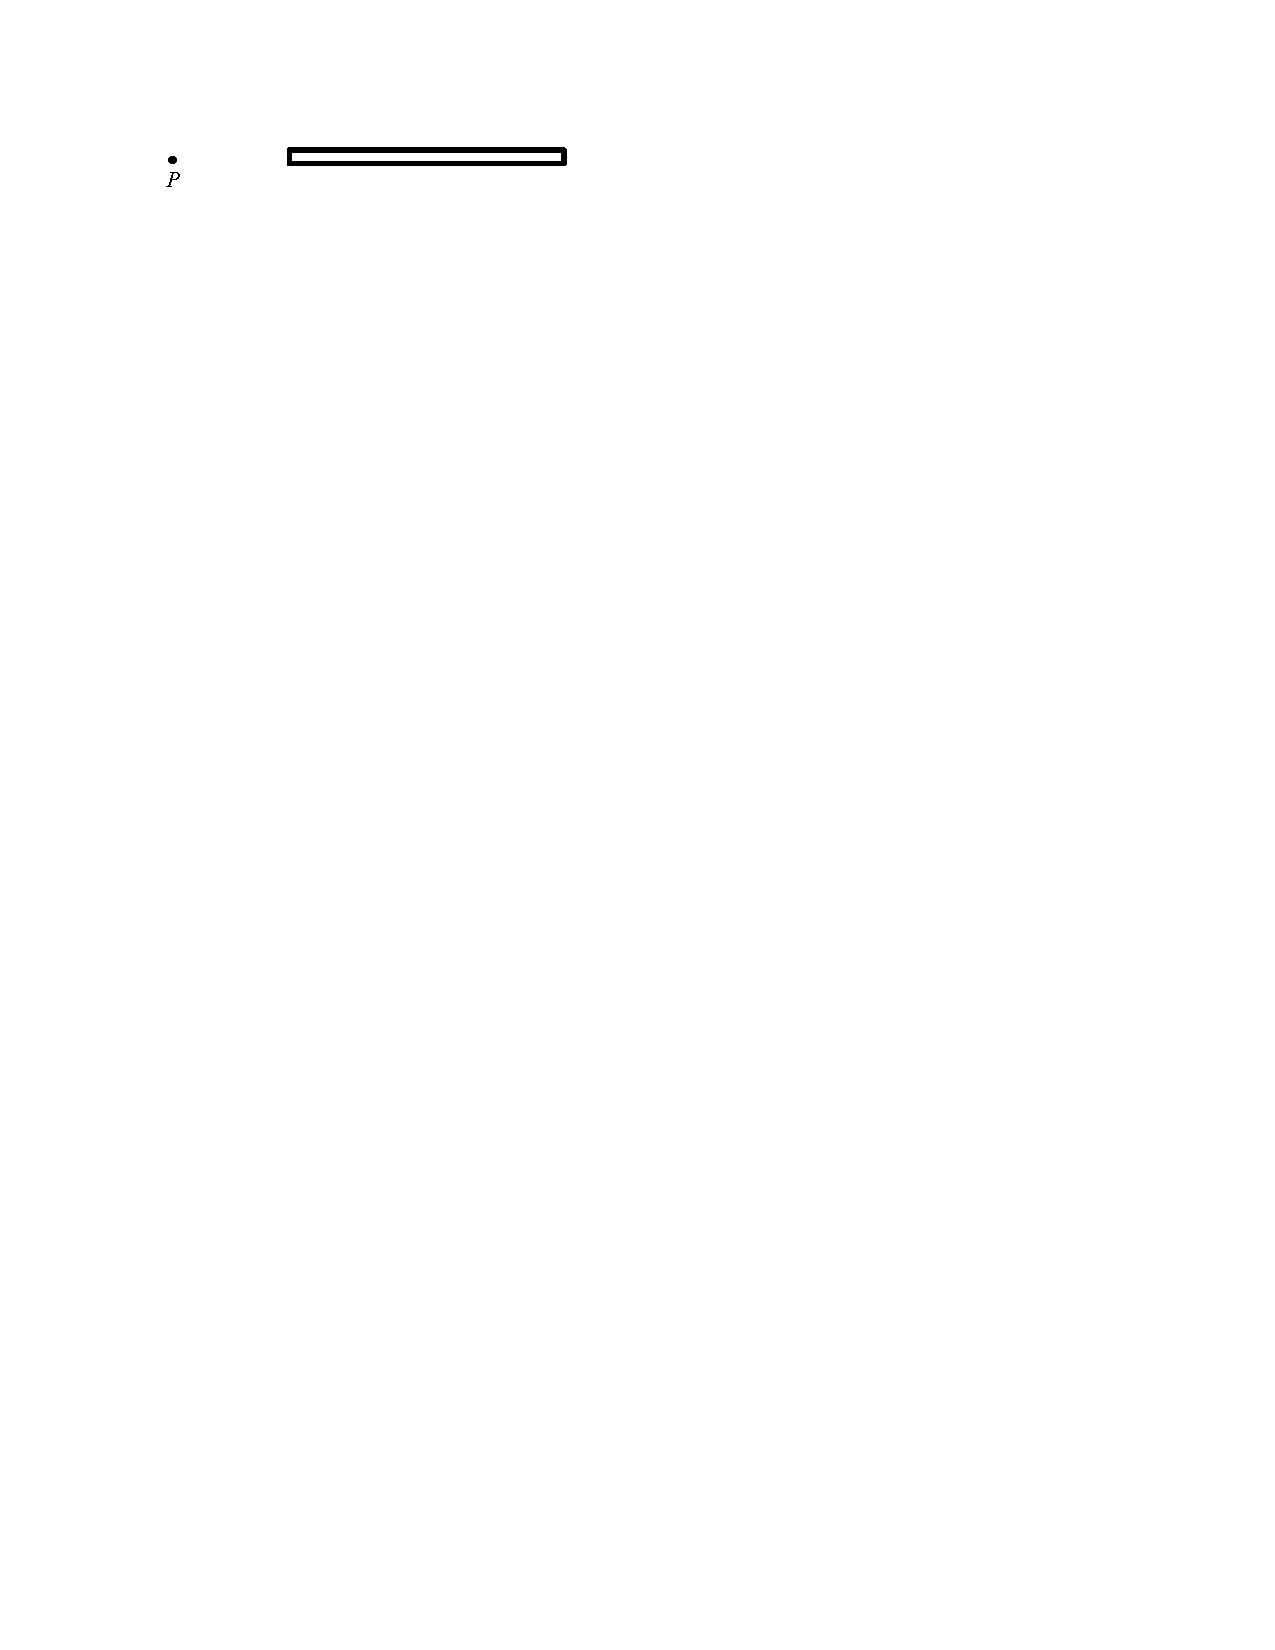
\includegraphics{M_problems/charges/point_on_rod_axis.pdf}
\end{center}
\end{Exercise}
\begin{Answer}
$\displaystyle E= \frac{k_e Q}{d(d+L)}$
\end{Answer}

%--------------------------------------------------------------------------------------------------------------
\figuretoright{0.30}[scale=0.85]{M_problems/charges/knight_23-36.pdf}{
\begin{Exercise}
(From Knight 4e, 23.36) What are the strength and direction of the electric field at the position indicated by the dot in the figure?  Give your answer (a)~in component form, and (b)~as a magnitude and angle measured cw or ccw from the positive $x$ axis.
\end{Exercise}
\begin{Answer}
(a) $(-9.7\hat{i}+9.2\hat{j}) \times 10^4$  N/C
\end{Answer}


%--------------------------------------------------------------------------------------------------------------
\begin{Exercise}
(From Knight 5e, 22.16) A small glass bead has been charged to $+20$~nC.  A small metal ball bearing 1.0~cm above the bead feels a 0.018~N electric force, pulling it downward.  What is the charge on the ball bearing?
\end{Exercise}
\begin{Answer}
10 nC
\end{Answer}
}
%--------------------------------------------------------------------------------------------------------------
\begin{Exercise}
(From Knight 5e, 22.29) The electric field at a point in space is $\vec{E}=(400\hat{i}+100\hat{j})$~N/C. 
\begin{enumerate}[labparts, nosep]
\item What is the electric force on a proton at this point? Give your answer in component form.
\item What is the electric force on an electron at this point? Give your answer in component form.
\item What is the magnitude of the proton's acceleration?
\item What is the magnitude of the electron's acceleration?
\end{enumerate}
\end{Exercise}
\begin{Answer}
(a)~$(6.4\hat{i}+1.6\hat{j})\times 10^{-17}$~N \\
(b)~$(-6.4\hat{i}-1.6\hat{j})\times 10^{-17}$~N \\
(c)~$4.0\times10^{10}$~m/s$^2$ \\
(d)~$7.3\times10^{13}$~m/s$^2$
\end{Answer}

%--------------------------------------------------------------------------------------------------------------
\begin{Exercise}
(a)~Write expressions for the surface area $A$ and the volume $V$ of a sphere of radius $R$. 
(b)~Write expressions for the surface area $A$ and the volume $V$ of a cylinder of radius $R$ and height $h$.  (If you already remember these, great!  If you need to look them up, fine.  Either way, we'll be needing these for class, so be sure you know them.)
\end{Exercise}



%--------------------------------------------------------------------------------------------------------------
\begin{Exercise}
(From Knight 5e, 22.27) What are the strength and direction of the electric field 1.0~mm away from (a)~a proton, and (b)~an electron?
\end{Exercise}
\begin{Answer}
(a) $1.4 \times 10^{-3}$~N/C away from the proton. (b)~$1.4 \times 10^{-3}$~N/C towards the electron.
\end{Answer}

%--------------------------------------------------------------------------------------------------------------
\figuretoright{0.27}[scale=0.85]{M_problems/charges/charges_in_cube.pdf}{
\begin{Exercise}
A cube with sides of length $L=0.1$~m has a particle with charge $Q=5.00~\mu$C located in its exact center.  
There are also six more identical charged particles, each with charge $q=-1.00~\mu$C, positioned symmetrically around the center as shown in the figure.  
Find the electric flux through \textit{one} face of the cube.
\end{Exercise}
\begin{Answer}
$-18.8$~kN$\cdot$m$^2$/C
\end{Answer}

%--------------------------------------------------------------------------------------------------------------
\begin{Exercise}
An infinitely long, solid cylinder of radius $R$ has a uniform charge density per volume of $\rho$.  
Find the electric field at a point inside the cylinder, a distance $r$ from its axis. 
\end{Exercise}
\begin{Answer}
$E = \rho r / 2 \epsilon_0$
\end{Answer}
}

%--------------------------------------------------------------------------------------------------------------
\begin{Exercise}
\label{rory_messed_up}
(a) A question on a physics quiz asks, 
\begin{quotation} 
``What is the electric field inside a sphere of uniform charge density $40$~nC/m$^3$ and radius $R=15$~cm, at a point 6~cm from the center.''
\end{quotation}  
Should your answer be given in terms of variables, or as a number?  (b)~A slightly different question on a physics quiz asks,
\begin{quotation} 
``What is the electric field inside a sphere of uniform charge density $\rho$ and radius $R$, at a point a distance $r$ from the center, where $r<R$.'' 
\end{quotation}  
What variables should be included in your answer?  
(c)~For the quiz question in~(b), should one's answer include the variable $Q$?  
(d)~Rory and Esmerelda took the quiz.  Esmerelda answered ``$E=\rho r/(3\epsilon_0)$.''  Rory answered ``$E=Qr / 4\pi \epsilon_0 R^3)$.'' Which student received full credit? 
(e)~How did Rory's answer make his physics instructor feel?  
(f)~Which student was accepted to graduate school in biogenetic chemical engineering science?  
(g)~Where does Rory work?  
(h)~Does Rory have any friends?  
(i)~Where does Rory live? 
(j)~What is the moral of Rory's cautionary tale?
\end{Exercise}
\begin{Answer}
(a) The answer should be given as a number, because the quantities in the problem were given as numerical values.\\ 
(b) The answer should give the field $E$ in terms of only $\rho, R,$ and $r$, plus any necessary constants like $\pi$ or $\epsilon_0$, so that a numerical answer could be calculated directly if the quantities given had been written as numerical values.\\
(c) No, the answer should not include the variable $Q$, because it was not a variable given in the problem.\\
(d) Esmerelda received full credit, because she gave her answer in terms of only the variables given in the problem.\\
(e) Rory's physics instructor was initially merely grumpy, but subsequently became abjectly depressed and withdrew from society.\\
(f) Clearly, only Esmerelda was accepted.  Furthermore, Rory's graduate school application was stapled to the bulletin board in the admissions office as a pointed reminder about the importance of answering problems using only the variables given in a problem.\\ 
(g) Rory has no job; all prospective employers shunned him after learning that he had given an answer in terms of variables not given in a problem.\\  
(h) Rory no longer has any friends.  They too shunned him after learning that he had given an answer in terms of variables not given in a problem.\\
(i) Rory now lives in a van, down by the river.\footnote{Also acceptable: ``Rory lives in a park, where he begs for food from the squirrels.''}\\
(j) The moral of the story is that one should always give one's answers in terms of the only variables given in the problem.  If the problem says ``$Q,$'' don't give an answer that uses $\rho$ instead.  If a problem describes only lengths $L$ and $d$, don't use a new length $x$ in your answer unless you also include the definition of $x$ in terms of $L$ and $d$.
\end{Answer}

%--------------------------------------------------------------------------------------------------------------
\begin{Exercise}
(a)~Imagine drawing a picture of a region near several large charged particles and representing the electric field with a series of field lines.
If an additional small, positively charged particle is placed in the area, will the path of that small particle follow the field lines?
If you're not sure, go ahead and make a guess and write it down.  
(b)~The coyote is running horizontally at speed $v_0=12$~m/s when he runs off the edge of a 50-meter high vertical cliff.
How far from the base of the cliff does the coyote land?  
(c)~A proton (mass $m_p=1.67\times10^{-27}$~kg, charge $+1.6\times10^{-19}$~C) has an initial horizontal speed $v_0=120{,}000$~m/s when it enters a region between two horizontal charged plates, entering 0.50~cm above the lower plate. 
In between the two plates, there is a uniform electric field $E=980$~N/C pointing vertically down.  How far from the entrance of the plates does the proton land?  
(d)~In part (c), did the path of the proton follow the field lines?
\begin{center}
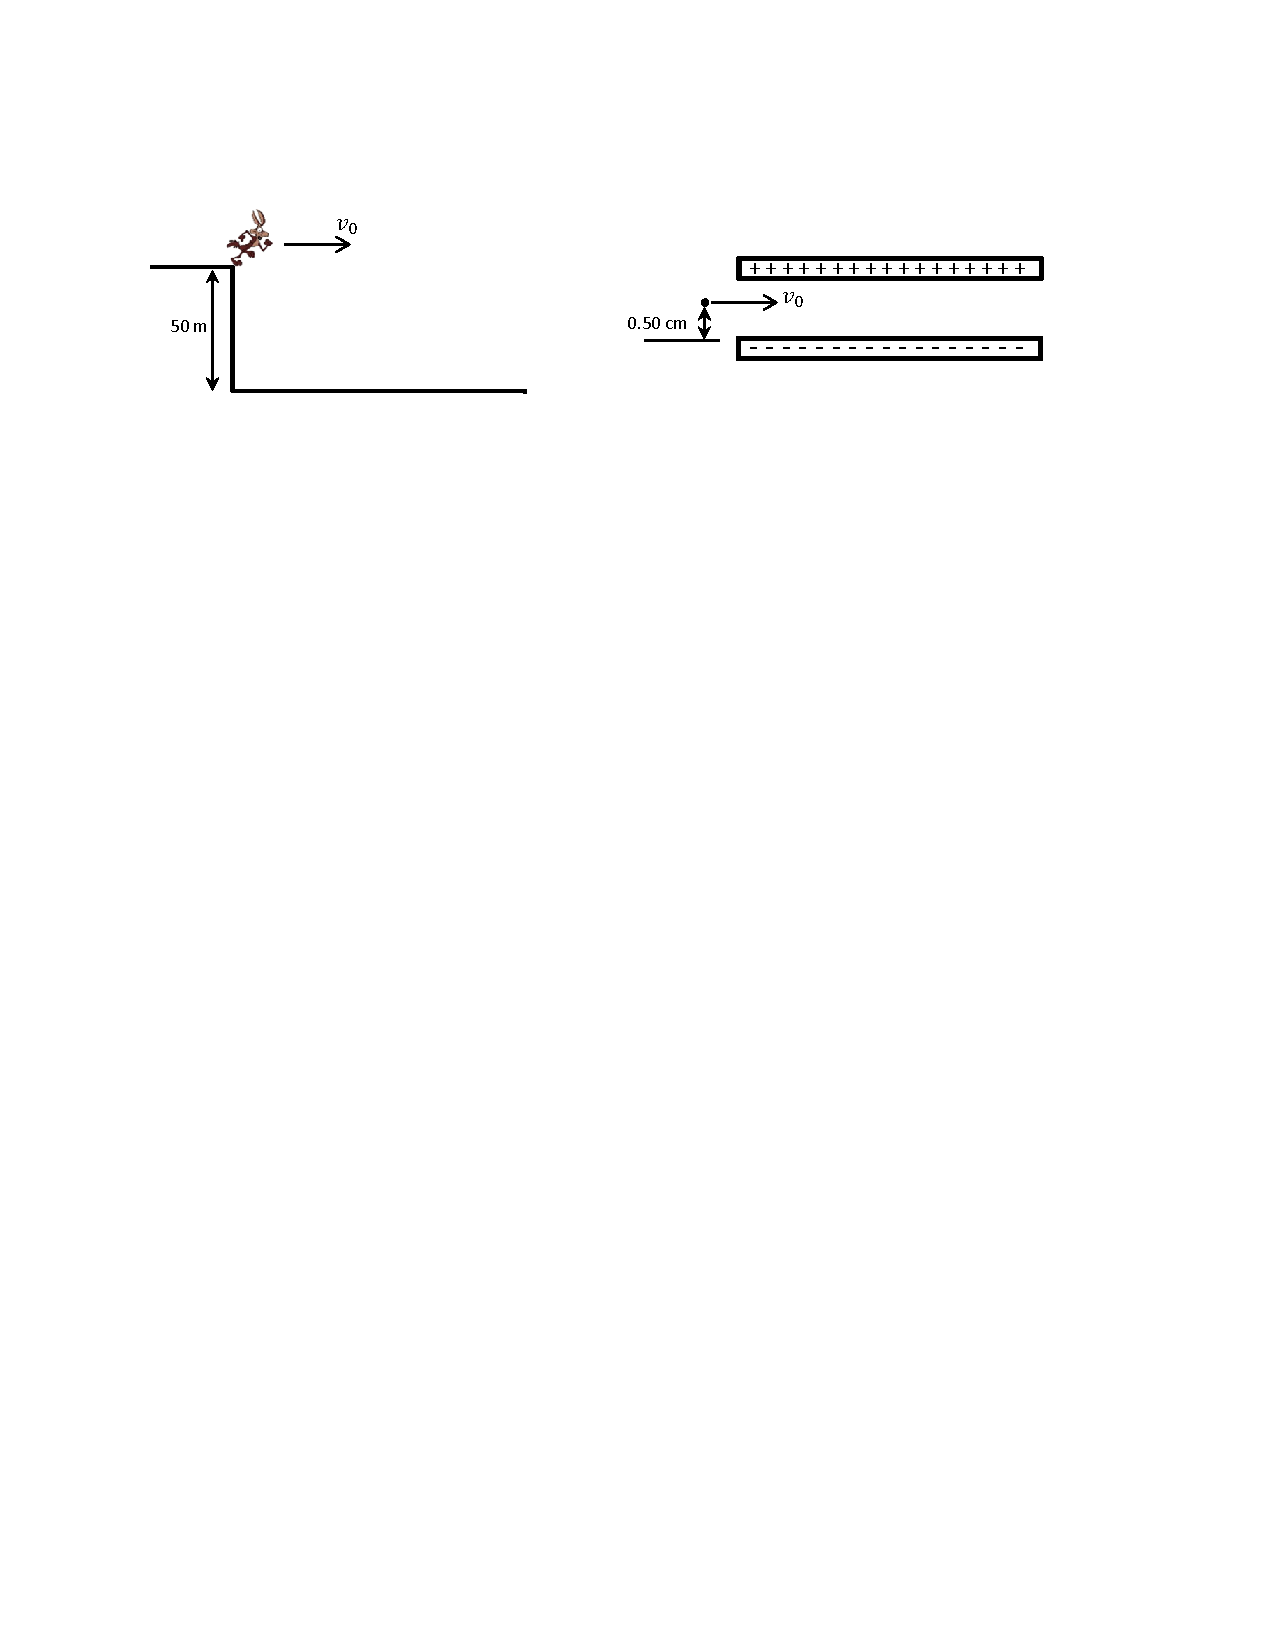
\includegraphics{M_problems/charges/coyote_and_capacitor.pdf}
\end{center}
\end{Exercise}
\begin{Answer}
(b) 38.3 meters (c)~39.1 mm (d)~Not so much.  At this point, you can go back and append your answer to part~(a), but do not erase all traces of your initial guess.  If the later parts of this problem have refined your understanding of part~(a), then so much the greater achievement!
\end{Answer}

%--------------------------------------------------------------------------------------------------------------
\figuretoright{0.16}[scale=0.95]{M_problems/charges/120_degree_arc.pdf}{
\begin{Exercise}
A sphere of radius $R$ carries a uniform charge density, such that its total charge is $Q$. 
Use Gauss' law to write the electric field $E$ at some place on the inside of the sphere, at some radius $r<R$.  
 (Note that this is exactly a problem we did in class, except that now you are given $Q$ instead of $\rho$, so your final answer must be in terms of $Q$ as well.  Don't be like Rory from problem~\ref{rory_messed_up}!)
\end{Exercise}
\begin{Answer}
$\displaystyle E=\frac{Qr}{4\pi \epsilon_0 R^3}$
\end{Answer}



%--------------------------------------------------------------------------------------------------------------
\begin{Exercise}
A thin, uniformly charged rod of total charge $+Q$ is bent into a 120$^\circ$ circular arc of radius $R$, as shown.  
Find the electric field at the center point $P$.   (Hint: make each bit o' charge $dq$ have a length $ds=R\,d\theta$, and do an integral over the angle $\theta$. 
\end{Exercise}
\begin{Answer}
$\displaystyle E = \frac{3 \sqrt{3} Q} {8 \pi^2 \epsilon_0 R^2}$ to the right
\end{Answer}
}

\newpage
%--------------------------------------------------------------------------------------------------------------
\begin{Exercise}
(a) An infinite plane with area-charge density $+\sigma$ is pictured below at the left.  
The numbered points 1, 2, and 3 are evenly spaced, and the plane lies midway between points 1 and 2. 
Find the electric field $\vec{E}$ at each of the three points, in terms of $\sigma, \epsilon_0$, and the unit vector$\hat{j}$. (This is a standard and familiar Gauss' law problem.)
\begin{center}
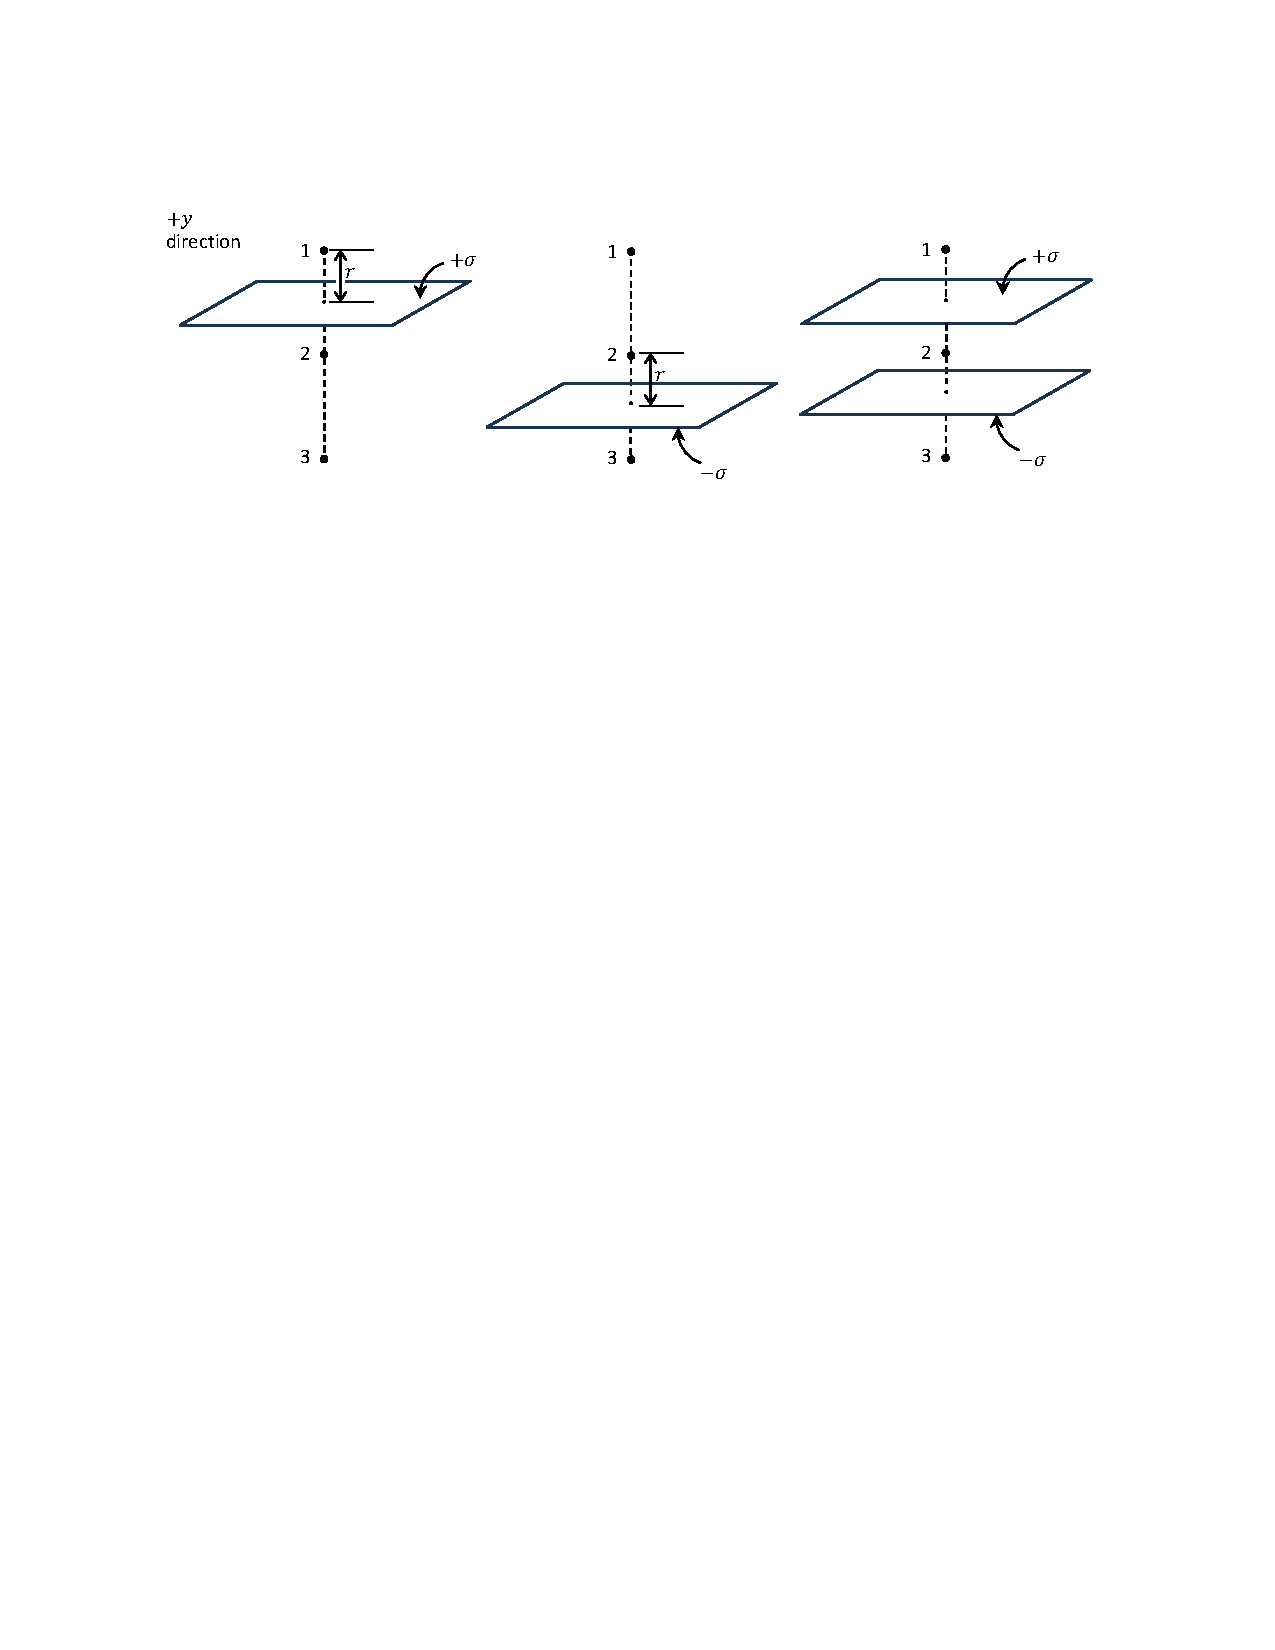
\includegraphics{M_problems/charges/superposition_of_planes.pdf}
\end{center}

(b) In the middle figure, the positively charged plane has been replaced by a different infinite plane betweem points 2 and 3, this time with charge density $-\sigma$.  Now what is the electric field $\vec{E}$ at each of the three points, again in terms of $\sigma, \epsilon_0$, and $\hat{j}$?  

(c) What is the electric field $\vec{E}$ at each of the three points in rightmost figure, with both the positive and negative plane?  (\textit{Hint: it's a little tricky to do this part from scratch using Gauss' law directly, but it's easy to do using your results of (a)~and (b)~and the idea of superposition.})
\end{Exercise}
\begin{Answer}
(a) $\vec{E_1}=+\frac{\sigma}{2\epsilon_0}\hat{j}, 
\vec{E_2}=-\frac{\sigma}{ 2\epsilon_0}\hat{j}, 
\vec{E_3}=-\frac{\sigma}{ 2\epsilon_0}\hat{j} $\\
(b) $\vec{E_1}=-\frac{\sigma}{2\epsilon_0}\hat{j}, 
\vec{E_2}=-\frac{\sigma}{ 2\epsilon_0}\hat{j}, 
\vec{E_3}=+\frac{\sigma}{ 2\epsilon_0}\hat{j} $\\
(c) $\vec{E_2}=-\frac{\sigma}{ \epsilon_0}\hat{j}, 
\vec{E_1}=\vec{E_3} =0$ 
\end{Answer}

%--------------------------------------------------------------------------------------------------------------
\figuretoright{0.42}[scale=0.95]{M_problems/charges/nested_spheres.pdf}{
\begin{Exercise}
The figure below shows a solid metal sphere at the center of a hollow metal shell.  
The electric fields $\vec{E_1}$ and $\vec{E_2}$ are both 15,000~N/C in magnitude, with directions as shown.  
What are the charges on each surface at 5~cm, 10~cm, and 15~cm?
\end{Exercise}
\begin{Answer}
The three surface charges are +10~nC, $-10$~nC, and $+48$~nC, not necessarily in that order.
\end{Answer}
}






\vspace{0.7in}

\textbf{Answers to Selected {\thesubsection} Problems:}
\label{charges_prob_answers}
%\shipoutExercise
\shipoutAnswer

\cleardoublepage
